\section{Results: Europe and United States}
\label{res}
We noted that none of the European SCs communicated about grid integration and demand response techniques with their associated ESPs. Additionally, there was little interest in a tighter integration with the ESPs.

Figures \ref{fig:USload} and \ref{fig:EUload} depict the total load in megawatts for each of the respondents in the United States and in Europe. Most supercomputing sites have a total load of under 5 MW (sixteen out of twenty). Four of the surveyed supercomputing sites had a total load of over 10 MW. 
\begin{figure}
\begin{center}
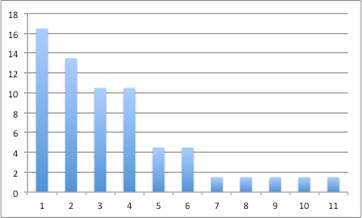
\includegraphics[scale=0.7]{figs/USLoad.jpg}
\caption{Total Load at at SCs in United States}
\label{fig:USload}
\end{center}
\end{figure}

\begin{figure}
\begin{center}
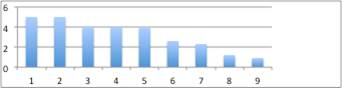
\includegraphics[scale=1]{figs/EULoad.jpg}
\caption{Total Load at at SCs in Europe}
\label{fig:EUload}
\end{center}
\end{figure}

Both United States and Europe had power swings and fluctuations of a few megawatts. In our questionnaire, we asked respondents to report the maximum variability that they have experienced in their SCs. The results of these for United States as well as Europe are shown in Figures \ref{fig:USvar} and \ref{fig:EUvar} respectively. In the United States, three of the eleven sites surveyed had maximum variability of over 5 MW. For our United States respondents, the minimal option for reporting this was ``Less than 3 MW'', because of which we could not capture less intense power swings. In the European survey, we allowed the respondents to provide a more accurate value, and as shown in Figure \ref{fig:EUvar}, we observed power swings in the range of half a megawatt to about 2 MW. Almost all of the respondents reported that this variability is due to maintenance cycles, and that it can be scheduled \emph{day-ahead} if necessary.

\begin{figure}
\begin{center}
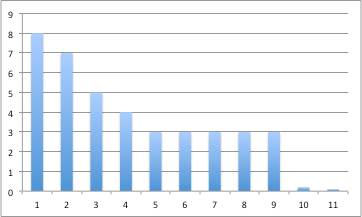
\includegraphics[scale=0.8]{figs/USVar.jpg}
\caption{Maximum Variability at at SCs in United States}
\label{fig:USvar}
\end{center}
\end{figure}

\begin{figure}
\begin{center}
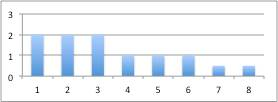
\includegraphics[scale=0.8]{figs/EUVar.jpg}
\caption{Maximum Variability at at SCs in Europe}
\label{fig:EUvar}
\end{center}
\end{figure}

